\section{Integrales triples en coordenadas cilíndricas}

Las coordenadas cilíndricas extienden las coordenadas polares del plano al espacio. Un punto se describe mediante la distancia $r$ de su proyección al eje $z$, el ángulo $\theta$ medido en el plano $xy$ desde el eje $x$ positivo y la altura $z$. La relación con las coordenadas cartesianas es
\[
x=r\cos\theta,\qquad y=r\sin\theta,\qquad z=z,
\]
con $r\geq0$. En sentido inverso,
\[
r=\sqrt{x^2+y^2},\qquad \tan\theta=\frac{y}{x},
\]
donde el cuadrante de $(x,y)$ determina el valor de $\theta$. En el eje $z$ se tiene $r=0$ y el ángulo no es único; esta falta de unicidad no afecta las integrales porque el eje tiene volumen cero.

Las superficies coordenadas permiten interpretar las cotas:
\begin{itemize}
    \item $r=c$ es un cilindro circular de radio $c$ alrededor del eje $z$;
    \item $\theta=\theta_0$ es un semiplano vertical que contiene al eje $z$;
    \item $z=c$ es un plano horizontal.
\end{itemize}
Por ello, estas coordenadas son adecuadas cuando la región contiene cilindros, conos, paraboloides de revolución o esferas alrededor del eje $z$.

\subsection{Sección de un cilindro genérico}

Una sección cilíndrica general queda determinada por dos radios, dos semiplanos angulares y dos alturas. Sean
\[
0\leq a<b,\qquad \alpha<\beta\leq\alpha+2\pi,
\qquad z_0<z_1.
\]
La región correspondiente es
\[
E=\left\{(r,\theta,z):a\leq r\leq b,\quad
\alpha\leq\theta\leq\beta,\quad z_0\leq z\leq z_1\right\}.
\]
Cuando $a>0$, sus fronteras radiales son dos cilindros concéntricos; cuando $a=0$, la región llega hasta el eje $z$. Los valores $\theta=\alpha$ y $\theta=\beta$ determinan los semiplanos laterales, mientras que $z=z_0$ y $z=z_1$ determinan la base y la tapa. La figura muestra que una caja rectangular en el espacio de parámetros $(r,\theta,z)$ se transforma en un sector cilíndrico anular.

\begingroup
\shorthandoff{>}
\begin{center}
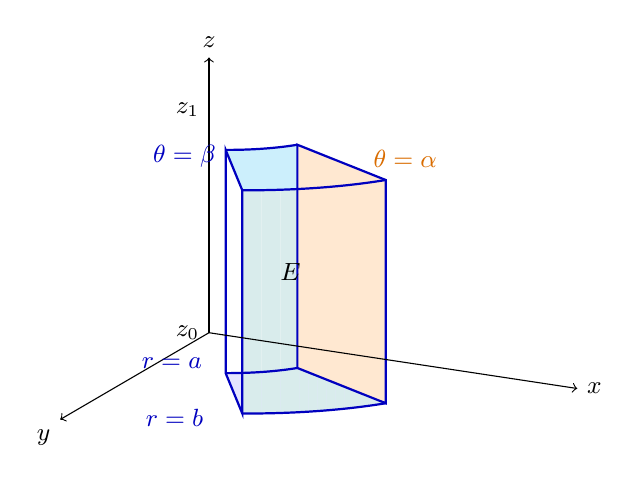
\begin{tikzpicture}[
    x={(1.65cm,-.25cm)},y={(-.72cm,-.42cm)},z={(0cm,.9cm)},
    scale=1.05,every node/.style={font=\small}]
    \def\rin{1}
    \def\rout{2}
    \def\za{0}
    \def\zb{3}
    \def\anga{30}
    \def\angb{60}

    \fill[blue!10]
        plot[domain=\anga:\angb,samples=35] ({\rout*cos(\x)},{\rout*sin(\x)},\za)
        -- plot[domain=\angb:\anga,samples=35] ({\rin*cos(\x)},{\rin*sin(\x)},\za) -- cycle;
    \fill[cyan!20]
        plot[domain=\anga:\angb,samples=35] ({\rout*cos(\x)},{\rout*sin(\x)},\zb)
        -- plot[domain=\angb:\anga,samples=35] ({\rin*cos(\x)},{\rin*sin(\x)},\zb) -- cycle;
    \foreach \i in {0,...,15} {
        \pgfmathsetmacro{\ta}{\anga+(\angb-\anga)*\i/16}
        \pgfmathsetmacro{\tb}{\anga+(\angb-\anga)*(\i+1)/16}
        \fill[teal!15]
            ({\rout*cos(\ta)},{\rout*sin(\ta)},\za) --
            ({\rout*cos(\tb)},{\rout*sin(\tb)},\za) --
            ({\rout*cos(\tb)},{\rout*sin(\tb)},\zb) --
            ({\rout*cos(\ta)},{\rout*sin(\ta)},\zb) -- cycle;
    }
    \fill[orange!18]
        ({\rin*cos(\anga)},{\rin*sin(\anga)},\za) --
        ({\rout*cos(\anga)},{\rout*sin(\anga)},\za) --
        ({\rout*cos(\anga)},{\rout*sin(\anga)},\zb) --
        ({\rin*cos(\anga)},{\rin*sin(\anga)},\zb) -- cycle;

    \foreach \rr in {\rin,\rout} {
        \draw[blue!75!black,thick]
            plot[domain=\anga:\angb,samples=40] ({\rr*cos(\x)},{\rr*sin(\x)},\za);
        \draw[blue!75!black,thick]
            plot[domain=\anga:\angb,samples=40] ({\rr*cos(\x)},{\rr*sin(\x)},\zb);
    }
    \foreach \tt in {\anga,\angb} {
        \draw[blue!75!black,thick]
            ({\rin*cos(\tt)},{\rin*sin(\tt)},\za) --
            ({\rout*cos(\tt)},{\rout*sin(\tt)},\za) --
            ({\rout*cos(\tt)},{\rout*sin(\tt)},\zb) --
            ({\rin*cos(\tt)},{\rin*sin(\tt)},\zb) -- cycle;
    }
    \draw[->] (0,0,0) -- (2.7,0,0) node[right] {$x$};
    \draw[->] (0,0,0) -- (0,2.5,0) node[below left] {$y$};
    \draw[->] (0,0,0) -- (0,0,3.7) node[above] {$z$};
    \node[blue!75!black, yshift=-40pt, xshift=-50pt] at ({2*cos(46)},{2*sin(46)},1.4) {$r=b$};
    \node[blue!75!black, yshift=-30pt, xshift=-25pt] at ({cos(54)},{sin(54)},1.25) {$r=a$};
    \node[orange!85!black, yshift=85pt, xshift=15pt] at ({1.75*cos(30)},{1.75*sin(30)},0) {$\theta=\alpha$};
    \node[blue!75!black, yshift=10pt, xshift=-20pt] at ({1.85*cos(60)},{1.85*sin(60)},3) {$\theta=\beta$};
    \node[left] at (0,0,0) {$z_0$};
    \node[left] at (0,0,3) {$z_1$};
    \node at ({1.5*cos(45)},{1.5*sin(45)},1.6) {$E$};
\end{tikzpicture}
\end{center}
\endgroup

Anticipando el diferencial $dV=r\,dr\,d\theta\,dz$, cuya deducción se presenta en el apartado siguiente, el volumen de esta región resulta
\begin{align*}
V
&=\int_{z_0}^{z_1}\int_\alpha^\beta\int_a^b
r\,dr\,d\theta\,dz\\
&=(z_1-z_0)(\beta-\alpha)\frac{b^2-a^2}{2}.
\end{align*}
Esta expresión reúne varios casos. Si $a=0$, se obtiene un sector de un cilindro macizo. Si $\beta-\alpha=2\pi$, se obtiene un cilindro anular completo; además, si $a=0$, su volumen se reduce a $\pi b^2(z_1-z_0)$.

\subsection{El diferencial de volumen}

Una celda cilíndrica pequeña está comprendida entre $r$ y $r+\Delta r$, entre $\theta$ y $\theta+\Delta\theta$, y entre $z$ y $z+\Delta z$. Sus dimensiones aproximadas son
\[
\Delta r,\qquad r\,\Delta\theta,\qquad \Delta z.
\]
La segunda longitud es la de un arco de radio $r$ y ángulo $\Delta\theta$. Por tanto,
\[
\Delta V\approx \Delta r\,(r\,\Delta\theta)\,\Delta z.
\]

\begingroup
\shorthandoff{>}
\begin{center}
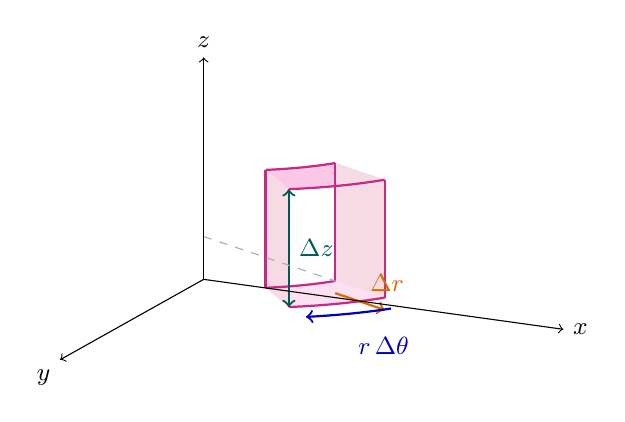
\begin{tikzpicture}[
    x={(1.8cm,-.25cm)},y={(-.75cm,-.42cm)},z={(0cm,1.8cm)},
    scale=1.08,every node/.style={font=\small}]
    \def\ra{1.25}
    \def\rb{1.72}
    \def\ta{28}
    \def\tb{50}
    \def\za{.28}
    \def\zb{1.05}

    \fill[magenta!12]
        plot[domain=\ta:\tb,samples=30] ({\rb*cos(\x)},{\rb*sin(\x)},\za)
        -- plot[domain=\tb:\ta,samples=30] ({\ra*cos(\x)},{\ra*sin(\x)},\za) -- cycle;
    \fill[magenta!22]
        plot[domain=\ta:\tb,samples=30] ({\rb*cos(\x)},{\rb*sin(\x)},\zb)
        -- plot[domain=\tb:\ta,samples=30] ({\ra*cos(\x)},{\ra*sin(\x)},\zb) -- cycle;
    \foreach \tt in {\ta,\tb} {
        \fill[purple!14]
            ({\ra*cos(\tt)},{\ra*sin(\tt)},\za) --
            ({\rb*cos(\tt)},{\rb*sin(\tt)},\za) --
            ({\rb*cos(\tt)},{\rb*sin(\tt)},\zb) --
            ({\ra*cos(\tt)},{\ra*sin(\tt)},\zb) -- cycle;
    }
    \foreach \rr in {\ra,\rb} {
        \draw[magenta!80!black,thick]
            plot[domain=\ta:\tb,samples=35] ({\rr*cos(\x)},{\rr*sin(\x)},\za);
        \draw[magenta!80!black,thick]
            plot[domain=\ta:\tb,samples=35] ({\rr*cos(\x)},{\rr*sin(\x)},\zb);
    }
    \foreach \tt in {\ta,\tb} {
        \foreach \rr in {\ra,\rb} {
            \draw[magenta!80!black,thick]
                ({\rr*cos(\tt)},{\rr*sin(\tt)},\za) --
                ({\rr*cos(\tt)},{\rr*sin(\tt)},\zb);
        }
    }
    \draw[->,orange!85!black,thick]
        ({\ra*cos(\ta)},{\ra*sin(\ta)},{\za-.08}) --
        ({\rb*cos(\ta)},{\rb*sin(\ta)},{\za-.08})
        node[midway,above right] {$\Delta r$};
    \draw[->,blue!75!black,thick]
        plot[domain=\ta+2:\tb-2,samples=25]
        ({1.86*cos(\x)},{1.86*sin(\x)},{\za-.03});
    \node[blue!75!black,right] at ({1.9*cos(40)},{1.9*sin(40)},.05)
        {$r\,\Delta\theta$};
    \draw[<->,teal!70!black,thick]
        ({\rb*cos(\tb)},{\rb*sin(\tb)},\za) --
        ({\rb*cos(\tb)},{\rb*sin(\tb)},\zb)
        node[midway,right] {$\Delta z$};
    \draw[dashed,gray!65] (0,0,\za) -- ({\ra*cos(\ta)},{\ra*sin(\ta)},\za);
    \draw[->] (0,0,0) -- (2.35,0,0) node[right] {$x$};
    \draw[->] (0,0,0) -- (0,2.25,0) node[below left] {$y$};
    \draw[->] (0,0,0) -- (0,0,1.45) node[above] {$z$};
\end{tikzpicture}
\end{center}
\endgroup

Al hacer tender a cero las dimensiones de la celda, se obtiene el elemento de volumen diferencial
\[
dV=r\,dr\,d\theta\,dz.
\]
El factor $r$ de $dV$ refleja que celdas con el mismo incremento angular son más anchas cuando se encuentran más lejos del eje $z$.

\begin{mytheorem}{Cambio a coordenadas cilíndricas}
Sea $E$ una región para la cual la transformación cilíndrica cubre cada punto una sola vez, salvo posiblemente puntos de la frontera. Si $f$ es integrable en $E$ y $E^*$ es la región correspondiente en el espacio $(r,\theta,z)$, entonces
\[
\iiint_E f(x,y,z)\,dV
=\iiint_{E^*}f(r\cos\theta,r\sin\theta,z)\,r\,dr\,d\theta\,dz,
\]
\end{mytheorem}

\subsection{Qué representa integrar respecto de cada variable}

En un bloque cilíndrico, la variable interior indica el recorrido elemental que se acumula primero. La figura representa los tres recorridos dentro de un cuarto de cilindro.

\begingroup
\shorthandoff{>}
\begin{center}
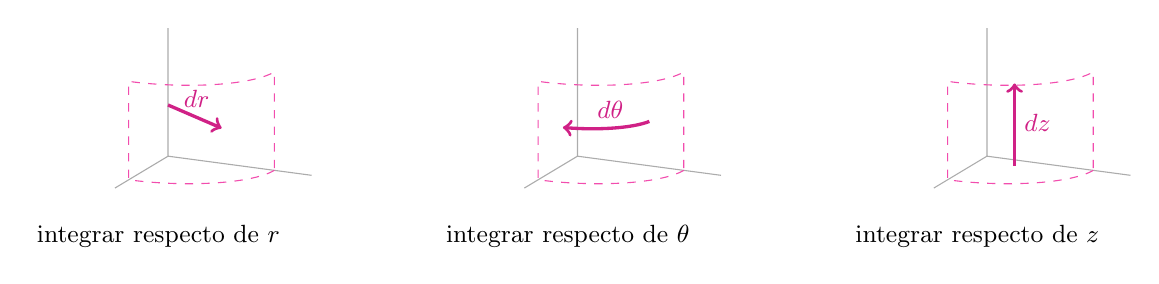
\begin{tikzpicture}[every node/.style={font=\small}]
    \begin{scope}[xshift=0cm,x={(1.35cm,-.18cm)},y={(-.5cm,-.3cm)},z={(0cm,1.25cm)}]
        \draw[gray!65] (0,0,0) -- (1.35,0,0) (0,0,0) -- (0,1.35,0) (0,0,0) -- (0,0,1.3);
        \draw[dashed,magenta!70]
            plot[domain=0:90,samples=30] ({cos(\x)},{sin(\x)},0)
            -- plot[domain=90:0,samples=30] ({cos(\x)},{sin(\x)},1) -- cycle;
        \draw[->,magenta!85!black,very thick] (0,0,.52) -- ({.9*cos(38)},{.9*sin(38)},.52);
        \node[magenta!85!black,above] at ({.48*cos(38)},{.48*sin(38)},.52) {$dr$};
        \node[below] at (.15,.65,-.42) {integrar respecto de $r$};
    \end{scope}
    \begin{scope}[xshift=5.2cm,x={(1.35cm,-.18cm)},y={(-.5cm,-.3cm)},z={(0cm,1.25cm)}]
        \draw[gray!65] (0,0,0) -- (1.35,0,0) (0,0,0) -- (0,1.35,0) (0,0,0) -- (0,0,1.3);
        \draw[dashed,magenta!70]
            plot[domain=0:90,samples=30] ({cos(\x)},{sin(\x)},0)
            -- plot[domain=90:0,samples=30] ({cos(\x)},{sin(\x)},1) -- cycle;
        \draw[->,magenta!85!black,very thick]
            plot[domain=8:80,samples=30] ({.72*cos(\x)},{.72*sin(\x)},.48);
        \node[magenta!85!black,above] at ({.72*cos(46)},{.72*sin(46)},.48) {$d\theta$};
        \node[below] at (.15,.65,-.42) {integrar respecto de $\theta$};
    \end{scope}
    \begin{scope}[xshift=10.4cm,x={(1.35cm,-.18cm)},y={(-.5cm,-.3cm)},z={(0cm,1.25cm)}]
        \draw[gray!65] (0,0,0) -- (1.35,0,0) (0,0,0) -- (0,1.35,0) (0,0,0) -- (0,0,1.3);
        \draw[dashed,magenta!70]
            plot[domain=0:90,samples=30] ({cos(\x)},{sin(\x)},0)
            -- plot[domain=90:0,samples=30] ({cos(\x)},{sin(\x)},1) -- cycle;
        \draw[->,magenta!85!black,very thick]
            ({.66*cos(48)},{.66*sin(48)},.08) --
            ({.66*cos(48)},{.66*sin(48)},.92);
        \node[magenta!85!black,right] at ({.66*cos(48)},{.66*sin(48)},.52) {$dz$};
        \node[below] at (.15,.65,-.42) {integrar respecto de $z$};
    \end{scope}
\end{tikzpicture}
\end{center}
\endgroup

Así, integrar respecto de $r$ recorre un segmento radial con $\theta$ y $z$ fijos; integrar respecto de $\theta$ recorre un arco con $r$ y $z$ fijos; e integrar respecto de $z$ recorre un segmento vertical con $r$ y $\theta$ fijos.

Una región simple respecto de $z$ suele escribirse como
\[
E^*=\{(r,\theta,z):\alpha\leq\theta\leq\beta,
\ g_1(\theta)\leq r\leq g_2(\theta),
\ u(r,\theta)\leq z\leq v(r,\theta)\}.
\]
En tal caso,
\[
\iiint_E f\,dV
=\int_\alpha^\beta\int_{g_1(\theta)}^{g_2(\theta)}
\int_{u(r,\theta)}^{v(r,\theta)}
f(r\cos\theta,r\sin\theta,z)\,r\,dz\,dr\,d\theta.
\]
Las cotas angulares se obtienen de los rayos que delimitan la proyección sobre $xy$; las cotas radiales se obtienen de sus curvas interior y exterior; y las cotas de $z$ se obtienen de las superficies inferior y superior. 

\paragraph{Ejemplo 1. Volumen de una esfera}

Sea $E$ la esfera de radio $a>0$ centrada en el origen:
\[
E=\{(x,y,z):x^2+y^2+z^2\leq a^2\}.
\]
Como $x^2+y^2=r^2$, para cada $r$ la coordenada vertical queda entre las dos semiesferas
\[
-\sqrt{a^2-r^2}\leq z\leq\sqrt{a^2-r^2}.
\]

\begingroup
\shorthandoff{>}
\begin{center}
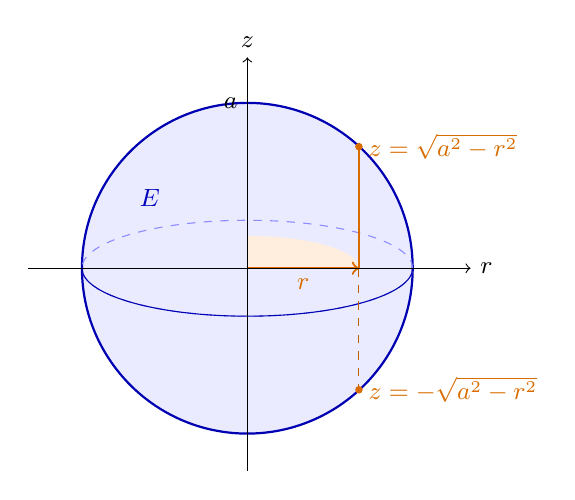
\begin{tikzpicture}[scale=1.05,every node/.style={font=\small}]
    \fill[blue!8] (0,0) circle (2cm);
    \draw[blue!70!black,thick] (0,0) circle (2cm);
    \draw[dashed,blue!45] (0,0) ellipse (2cm and .58cm);
    \draw[blue!70!black] (-2,0) arc[start angle=180,end angle=360,x radius=2cm,y radius=.58cm];
    \fill[orange!13] (0,0) -- (1.35,0) arc[start angle=0,end angle=90,x radius=1.35cm,y radius=.39cm] -- cycle;
    \draw[->,orange!85!black,thick] (0,0) -- (1.35,0) node[midway,below] {$r$};
    \draw[orange!85!black,thick] (1.35,0) -- (1.35,1.47);
    \draw[dashed,orange!75!black] (1.35,0) -- (1.35,-1.47);
    \fill[orange!85!black] (1.35,1.47) circle (1.3pt);
    \fill[orange!85!black] (1.35,-1.47) circle (1.3pt);
    \draw[->] (-2.65,0) -- (2.7,0) node[right] {$r$};
    \draw[->] (0,-2.45) -- (0,2.55) node[above] {$z$};
    \node[right,orange!85!black] at (1.35,1.47) {$z=\sqrt{a^2-r^2}$};
    \node[right,orange!85!black] at (1.35,-1.47) {$z=-\sqrt{a^2-r^2}$};
    \node[left] at (0,2) {$a$};
    \node[blue!75!black] at (-1.18,.85) {$E$};
\end{tikzpicture}
\end{center}
\endgroup

El ángulo debe recorrer una vuelta completa y $0\leq r\leq a$. Por tanto,
\begin{align*}
V
&=\int_0^{2\pi}\int_0^a
\int_{-\sqrt{a^2-r^2}}^{\sqrt{a^2-r^2}}
r\,dz\,dr\,d\theta\\
&=2\pi\int_0^a2r\sqrt{a^2-r^2}\,dr.
\end{align*}
Con $u=a^2-r^2$ y $du=-2r\,dr$ se obtiene
\[
V=2\pi\left[ -\frac{2}{3}(a^2-r^2)^{3/2}\right]_0^a
=\frac{4\pi a^3}{3}.
\]

\paragraph{Ejemplo 2. Masa de un cono con densidad variable}

Se considera el cono recto de altura $h$ y radio de base $R$, con vértice en $(0,0,h)$ y base en $z=0$. Su densidad depende de la altura:
\[
\rho(r,\theta,z)=\rho_0\left(1+\frac{z}{h}\right),
\qquad \rho_0>0.
\]
En un corte de altura $z$, el radio del cono es $R(1-z/h)$.

\begingroup
\shorthandoff{>}
\begin{center}
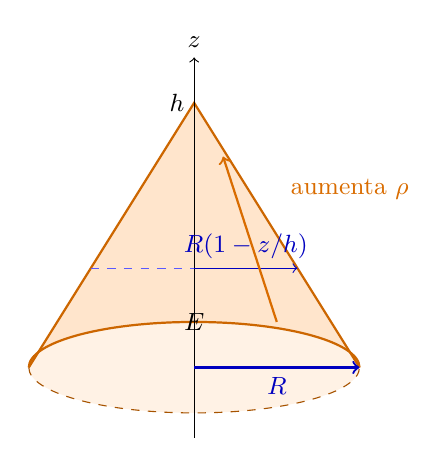
\begin{tikzpicture}[scale=1.05,every node/.style={font=\small}]
    \fill[orange!10] (-2,0) arc[start angle=180,end angle=360,x radius=2cm,y radius=.55cm]
        -- (0,3.2) -- cycle;
    \fill[orange!20] (-2,0) arc[start angle=180,end angle=0,x radius=2cm,y radius=.55cm]
        -- (0,3.2) -- cycle;
    \draw[orange!80!black,thick] (-2,0) -- (0,3.2) -- (2,0);
    \draw[dashed,orange!65!black] (-2,0) arc[start angle=180,end angle=360,x radius=2cm,y radius=.55cm];
    \draw[orange!80!black,thick] (-2,0) arc[start angle=180,end angle=0,x radius=2cm,y radius=.55cm];
    \draw[->] (0,-.85) -- (0,3.75) node[above] {$z$};
    \draw[->,blue!75!black,thick] (0,0) -- (2,0) node[midway,below] {$R$};
    \draw[dashed,blue!65] (-1.25,1.2) -- (1.25,1.2);
    \draw[->,blue!75!black] (0,1.2) -- (1.25,1.2)
        node[midway,above] {$R(1-z/h)$};
    \node[left] at (0,3.2) {$h$};
    \node[orange!85!black,right] at (1.05,2.15) {aumenta $\rho$};
    \draw[->,orange!85!black,thick] (1.0,.55) -- (.35,2.55);
    \node at (0,.55) {$E$};
\end{tikzpicture}
\end{center}
\endgroup

La masa se obtiene de
\begin{align*}
m
&=\int_0^h\int_0^{2\pi}\int_0^{R(1-z/h)}
\rho_0\left(1+\frac{z}{h}\right)r\,dr\,d\theta\,dz\\
&=\pi\rho_0R^2\int_0^h
\left(1+\frac{z}{h}\right)\left(1-\frac{z}{h}\right)^2dz.
\end{align*}
Al usar $t=z/h$,
\begin{align*}
m
&=\pi\rho_0R^2h\int_0^1(1+t)(1-t)^2\,dt\\
&=\pi\rho_0R^2h\int_0^1(1-t-t^2+t^3)\,dt
=\frac{5\pi\rho_0R^2h}{12}.
\end{align*}

\paragraph{Ejemplo 3. Momentos de inercia de un cilindro}

Sea un cilindro circular homogéneo de radio $R$, altura $h$ y masa $M$, centrado en el origen y con eje sobre $z$. Su volumen es $\pi R^2h$, de modo que la densidad constante es
\[
\rho_0=\frac{M}{\pi R^2h}.
\]

\begingroup
\shorthandoff{>}
\begin{center}
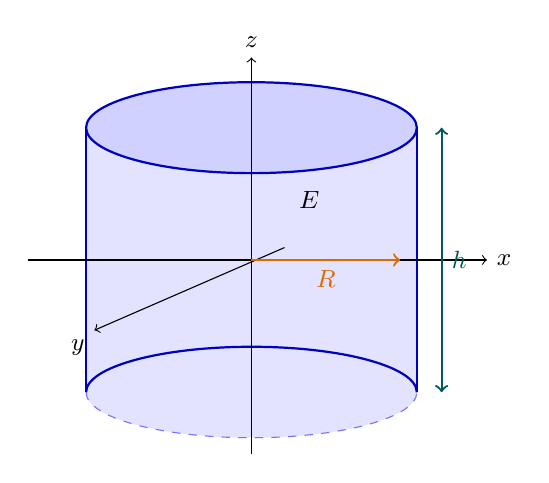
\begin{tikzpicture}[scale=1.05,every node/.style={font=\small}]
    \fill[blue!11] (-2,-1.6) -- (-2,1.6)
        arc[start angle=180,end angle=360,x radius=2cm,y radius=.55cm]
        -- (2,-1.6) arc[start angle=0,end angle=-180,x radius=2cm,y radius=.55cm] -- cycle;
    \fill[blue!18] (0,1.6) ellipse (2cm and .55cm);
    \draw[blue!75!black,thick] (-2,-1.6) -- (-2,1.6)
        (2,-1.6) -- (2,1.6);
    \draw[blue!75!black,thick] (0,1.6) ellipse (2cm and .55cm);
    \draw[dashed,blue!55] (-2,-1.6) arc[start angle=180,end angle=360,x radius=2cm,y radius=.55cm];
    \draw[blue!75!black,thick] (-2,-1.6) arc[start angle=180,end angle=0,x radius=2cm,y radius=.55cm];
    \draw[->] (-2.7,0) -- (2.85,0) node[right] {$x$};
    \draw[->] (0,-2.35) -- (0,2.45) node[above] {$z$};
    \draw[->] (.4,.15) -- (-1.9,-.85) node[below left] {$y$};
    \draw[->,orange!85!black,thick] (0,0) -- (1.8,0)
        node[midway,below] {$R$};
    \draw[<->,teal!70!black,thick] (2.3,-1.6) -- (2.3,1.6)
        node[midway,right] {$h$};
    \node at (.7,.72) {$E$};
\end{tikzpicture}
\end{center}
\endgroup

La distancia al eje $z$ es $r$, por lo que
\begin{align*}
I_z
&=\iiint_E r^2\rho_0\,dV
=\rho_0\int_{-h/2}^{h/2}\int_0^{2\pi}\int_0^R r^3\,dr\,d\theta\,dz\\
&=\rho_0h(2\pi)\frac{R^4}{4}
=\frac12MR^2.
\end{align*}
Para el eje $x$, la distancia al cuadrado es $y^2+z^2=r^2\sin^2\theta+z^2$. Entonces
\begin{align*}
I_x
&=\rho_0\int_{-h/2}^{h/2}\int_0^{2\pi}\int_0^R
(r^2\sin^2\theta+z^2)r\,dr\,d\theta\,dz\\
&=\rho_0\left(
h\cdot\pi\cdot\frac{R^4}{4}
+\frac{h^3}{12}\cdot2\pi\cdot\frac{R^2}{2}
\right)\\
&=\frac{M}{12}(3R^2+h^2).
\end{align*}
La simetría alrededor del eje $z$ implica $I_y=I_x$. Por tanto, los tres momentos son
\[
I_x=I_y=\frac{M}{12}(3R^2+h^2),
\qquad I_z=\frac12MR^2.
\]

\section{Integrales triples en coordenadas esféricas}

Las coordenadas esféricas permiten describir un sólido mediante distancias al origen y direcciones. Son adecuadas para regiones limitadas por esferas centradas en el origen y conos con vértice en él, y para funciones que dependen de $x^2+y^2+z^2$. En estos casos, las fronteras y el integrando suelen adquirir expresiones más sencillas, lo que facilita el cálculo de volúmenes, masas y centros de masa.

En coordenadas esféricas, un punto se representa mediante $(\rho,\theta,\varphi)$, donde $\rho$ es su distancia al origen, $\theta$ es el ángulo de su proyección sobre $xy$ medido desde el eje $x$ positivo y $\varphi$ es el ángulo medido desde el eje $z$ positivo. Se toma
\[
\rho\geq0,\qquad 0\leq\theta<2\pi,\qquad 0\leq\varphi\leq\pi.
\]
La relación con las coordenadas cartesianas es
\[
x=\rho\sin\varphi\cos\theta,\qquad
y=\rho\sin\varphi\sin\theta,\qquad z=\rho\cos\varphi.
\]
Y viceversa,
\[
\rho=\sqrt{x^2+y^2+z^2},\qquad
r=\sqrt{x^2+y^2}=\rho\sin\varphi.
\]

La distancia $\rho$ se mide desde el origen, mientras que $r$ se mide desde el eje $z$. Para $\rho>0$, se tiene $\varphi=\arccos(z/\rho)$; el ángulo $\theta$ se determina con el cuadrante de $(x,y)$. En el eje $z$, $\theta$ no es único, y en el origen tampoco lo es $\varphi$. Estos conjuntos tienen volumen cero y no afectan las integrales. En esta sección la densidad de masa se denota por $\rho_m$, para distinguirla de la coordenada radial $\rho$.

Las superficies coordenadas explican la forma de las cotas:
\begin{itemize}
    \item $\rho=c$, con $c>0$, es una esfera centrada en el origen;
    \item $\theta=\theta_0$ es un semiplano vertical que contiene al eje $z$;
    \item $\varphi=\varphi_0$, con $0<\varphi_0<\pi/2$, es la hoja superior de un cono circular; si $\pi/2<\varphi_0<\pi$, es una hoja inferior. Para $\varphi_0=\pi/2$ se obtiene el plano $xy$, y para $\varphi_0=0,\pi$ se obtienen los semiejes de $z$.
\end{itemize}

\subsection{Sección de una esfera genérica}

Sean
\[
0\leq a<b,\qquad \alpha<\beta\leq\alpha+2\pi,
\qquad 0\leq\varphi_0<\varphi_1\leq\pi.
\]
Se considera el bloque esférico cuya región de parámetros es
\[
E^*=\{(\rho,\theta,\varphi):a\leq\rho\leq b,\quad
\alpha\leq\theta\leq\beta,\quad
\varphi_0\leq\varphi\leq\varphi_1\}.
\]
Su imagen $E$ está comprendida entre dos esferas, dos semiplanos y dos superficies de ángulo polar constante. Cuando $a=0$, llega al origen. Esta sección se delimita mediante radios y ángulos; un segmento esférico limitado por planos paralelos tiene, en general, cotas radiales que dependen de $\varphi$.

\begingroup
\shorthandoff{>}
\begin{center}
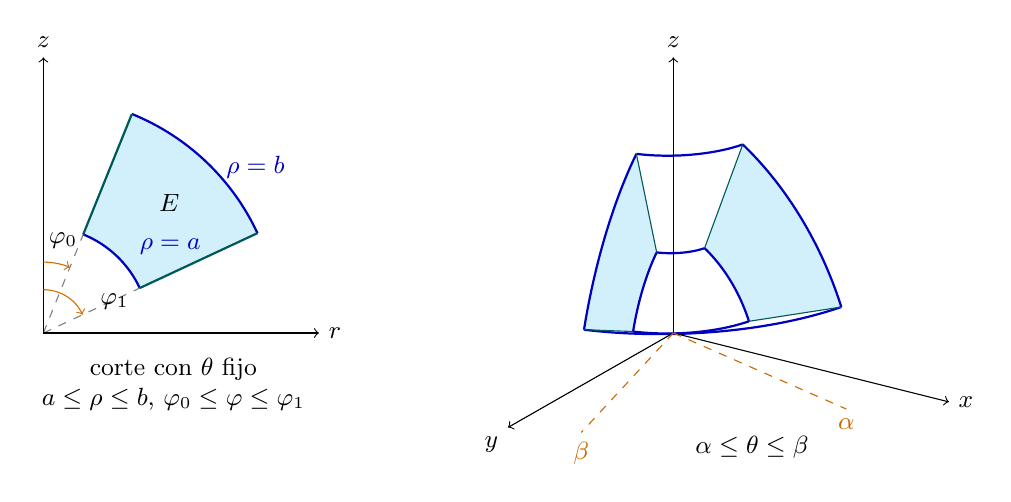
\begin{tikzpicture}[every node/.style={font=\small}]
    % Corte meridiano: las dos esferas se convierten en arcos concéntricos.
    \begin{scope}
        \fill[cyan!18] plot[domain=22:65,samples=40] ({3*sin(\x)},{3*cos(\x)})
            -- plot[domain=65:22,samples=40] ({1.35*sin(\x)},{1.35*cos(\x)}) -- cycle;
        \foreach \rr in {1.35,3} {
            \draw[blue!75!black,thick] plot[domain=22:65,samples=40]
                ({\rr*sin(\x)},{\rr*cos(\x)});
        }
        \foreach \pp in {22,65} {
            \draw[dashed,gray] (0,0) -- ({1.35*sin(\pp)},{1.35*cos(\pp)});
            \draw[teal!70!black,thick] ({1.35*sin(\pp)},{1.35*cos(\pp)})
                -- ({3*sin(\pp)},{3*cos(\pp)});
        }
        \draw[->] (0,0) -- (3.5,0) node[right] {$r$};
        \draw[->] (0,0) -- (0,3.5) node[above] {$z$};
        \draw[->,orange!85!black] (0,.9) arc[start angle=90,end angle=68,radius=.9];
        \node[above] at (.25,.95) {$\varphi_0$};
        \draw[->,orange!85!black] (0,.55) arc[start angle=90,end angle=25,radius=.55];
        \node[right] at (.6,.4) {$\varphi_1$};
        \node[right,blue!75!black] at (1.1,1.1) {$\rho=a$};
        \node[right,blue!75!black] at (2.2,2.1) {$\rho=b$};
        \node at (1.6,1.65) {$E$};
        \node[align=center] at (1.65,-.65) {corte con $\theta$ fijo\\$a\leq\rho\leq b$, $\varphi_0\leq\varphi\leq\varphi_1$};
    \end{scope}
    % El giro del corte meridiano produce el bloque espacial.
    \begin{scope}[xshift=8cm,x={(1cm,-.25cm)},y={(-.7cm,-.4cm)},z={(0cm,1cm)}]
        \foreach \tt in {15,75} {
            \fill[cyan!18] plot[domain=22:65,samples=35]
                ({3*sin(\x)*cos(\tt)},{3*sin(\x)*sin(\tt)},{3*cos(\x)})
                -- plot[domain=65:22,samples=35]
                ({1.35*sin(\x)*cos(\tt)},{1.35*sin(\x)*sin(\tt)},{1.35*cos(\x)}) -- cycle;
        }
        \foreach \rr in {1.35,3} {
            \foreach \pp in {22,65} {
                \draw[blue!75!black,thick] plot[domain=15:75,samples=40]
                    ({\rr*sin(\pp)*cos(\x)},{\rr*sin(\pp)*sin(\x)},{\rr*cos(\pp)});
            }
            \foreach \tt in {15,75} {
                \draw[blue!75!black,thick] plot[domain=22:65,samples=40]
                    ({\rr*sin(\x)*cos(\tt)},{\rr*sin(\x)*sin(\tt)},{\rr*cos(\x)});
            }
        }
        \foreach \tt in {15,75} {
            \foreach \pp in {22,65} {
                \draw[teal!70!black] ({1.35*sin(\pp)*cos(\tt)},{1.35*sin(\pp)*sin(\tt)},{1.35*cos(\pp)})
                    -- ({3*sin(\pp)*cos(\tt)},{3*sin(\pp)*sin(\tt)},{3*cos(\pp)});
            }
        }
        \draw[->] (0,0,0) -- (3.5,0,0) node[right] {$x$};
        \draw[->] (0,0,0) -- (0,3,0) node[below left] {$y$};
        \draw[->] (0,0,0) -- (0,0,3.5) node[above] {$z$};
        \foreach \tt/\lab in {15/\alpha,75/\beta} {
            \draw[dashed,orange!80!black] (0,0,0) -- ({2.8*cos(\tt)},{2.8*sin(\tt)},0)
                node[below] {$\lab$};
        }
        \node at (1,0,-1.2) {$\alpha\leq\theta\leq\beta$};
    \end{scope}
\end{tikzpicture}
\end{center}
\endgroup

Considerando el diferencial que se justificará más adelante, el volumen es
\begin{align*}
V&=\int_\alpha^\beta\int_{\varphi_0}^{\varphi_1}\int_a^b
\rho^2\sin\varphi\,d\rho\,d\varphi\,d\theta\\
&=(\beta-\alpha)\frac{b^3-a^3}{3}
(\cos\varphi_0-\cos\varphi_1).
\end{align*}
Por ejemplo, $a=0$, $b=R$, $\beta-\alpha=2\pi$, $\varphi_0=0$ y $\varphi_1=\pi$ describen la esfera maciza completa, cuyo volumen resulta $4\pi R^3/3$.

\subsection{El diferencial de volumen esférico}

Una celda pequeña queda comprendida entre $\rho$ y $\rho+\Delta\rho$, entre $\varphi$ y $\varphi+\Delta\varphi$ y entre $\theta$ y $\theta+\Delta\theta$. Sus tres dimensiones aproximadas, con los ángulos medidos en radianes, son
\[
\Delta\rho,\qquad \rho\,\Delta\varphi,\qquad
\rho\sin\varphi\,\Delta\theta.
\]
La primera es un espesor radial. La segunda es un arco azimutal sobre una esfera de radio $\rho$. La tercera es un arco de paralelo: al mantener $\rho$ y $\varphi$ fijos, el punto gira alrededor del eje $z$ en una circunferencia de radio $r=\rho\sin\varphi$.

\begingroup
\shorthandoff{>}
\begin{center}
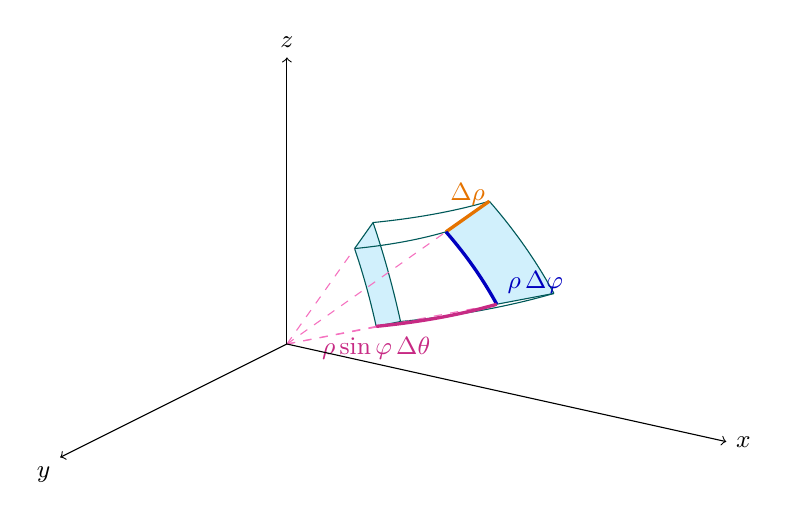
\begin{tikzpicture}[every node/.style={font=\small},
    x={(1.8cm,-.4cm)},y={(-1.2cm,-.6cm)},z={(0cm,1.3cm)}]
    \foreach \tt in {15,40} {
        \fill[cyan!18] plot[domain=40:58,samples=30]
            ({2.8*sin(\x)*cos(\tt)},{2.8*sin(\x)*sin(\tt)},{2.8*cos(\x)})
            -- plot[domain=58:40,samples=30]
            ({2.2*sin(\x)*cos(\tt)},{2.2*sin(\x)*sin(\tt)},{2.2*cos(\x)}) -- cycle;
    }
    \foreach \rr in {2.2,2.8} {
        \foreach \pp in {40,58} {
            \draw[teal!70!black] plot[domain=15:40,samples=30]
                ({\rr*sin(\pp)*cos(\x)},{\rr*sin(\pp)*sin(\x)},{\rr*cos(\pp)});
        }
        \foreach \tt in {15,40} {
            \draw[teal!70!black] plot[domain=40:58,samples=30]
                ({\rr*sin(\x)*cos(\tt)},{\rr*sin(\x)*sin(\tt)},{\rr*cos(\x)});
        }
    }
    \foreach \tt in {15,40} {
        \foreach \pp in {40,58} {
            \draw[dashed,magenta!55] (0,0,0) --
                ({2.2*sin(\pp)*cos(\tt)},{2.2*sin(\pp)*sin(\tt)},{2.2*cos(\pp)});
            \draw[teal!70!black]
                ({2.2*sin(\pp)*cos(\tt)},{2.2*sin(\pp)*sin(\tt)},{2.2*cos(\pp)}) --
                ({2.8*sin(\pp)*cos(\tt)},{2.8*sin(\pp)*sin(\tt)},{2.8*cos(\pp)});
        }
    }
    \draw[orange!90!black,very thick]
        ({2.2*sin(40)*cos(15)},{2.2*sin(40)*sin(15)},{2.2*cos(40)}) --
        ({2.8*sin(40)*cos(15)},{2.8*sin(40)*sin(15)},{2.8*cos(40)})
        node[midway,above] {$\Delta\rho$};
    \draw[blue!75!black,very thick] plot[domain=40:58,samples=30]
        ({2.2*sin(\x)*cos(15)},{2.2*sin(\x)*sin(15)},{2.2*cos(\x)})
        node[above right] {$\rho\,\Delta\varphi$};
    \draw[magenta!80!black,very thick] plot[domain=15:40,samples=30]
        ({2.2*sin(58)*cos(\x)},{2.2*sin(58)*sin(\x)},{2.2*cos(58)})
        node[below] {$\rho\sin\varphi\,\Delta\theta$};
    \draw[->] (0,0,0) -- (3.1,0,0) node[right] {$x$};
    \draw[->] (0,0,0) -- (0,2.4,0) node[below left] {$y$};
    \draw[->] (0,0,0) -- (0,0,2.8) node[above] {$z$};
\end{tikzpicture}
\end{center}
\endgroup

Las direcciones radial, meridiana y azimutal son perpendiculares entre sí en cada punto donde $\rho>0$ y $0<\varphi<\pi$. Por ello se puede aproximar su diferencial a un cubo con dimensiones
\[
\Delta V\approx(\Delta\rho)(\rho\,\Delta\varphi)
(\rho\sin\varphi\,\Delta\theta)
=\rho^2\sin\varphi\,\Delta\rho\,\Delta\varphi\,\Delta\theta.
\]
Tendiendo el límite de sus dimensiones a cero, el diferencial de volumen correspondiente es
\[
dV=\rho^2\sin\varphi\,d\rho\,d\varphi\,d\theta.
\]

\begin{mytheorem}{Cambio a coordenadas esféricas}
Sea $E$ una región sólida acotada, con frontera de volumen cero, y sea $E^*$ su región de parámetros esféricos. Si $f$ es continua en $E$, entonces
\begin{align*}
\iiint_E f(x,y,z)\,dV
&=\iiint_{E^*}f(\rho\sin\varphi\cos\theta,
\rho\sin\varphi\sin\theta,\rho\cos\varphi)\rho^2\sin\varphi\,d\rho\,d\varphi\,d\theta.
\end{align*}
\end{mytheorem}

\subsection{Qué representa variar cada coordenada}

Con las otras dos coordenadas fijas, cada variable describe un recorrido distinto: $\rho$ recorre un segmento radial, $\varphi$ recorre un arco azimutal y $\theta$ recorre un arco de paralelo. La figura muestra estos recorridos sobre una esfera de radio $R$; las flechas indican el sentido de aumento.

\begingroup
\shorthandoff{>}
\begin{center}
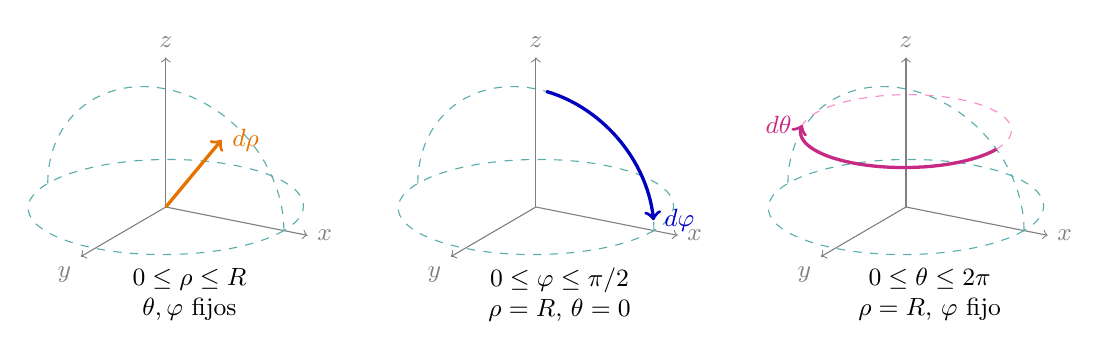
\begin{tikzpicture}[every node/.style={font=\small}]
    \foreach \panel in {0,1,2} {
        \begin{scope}[xshift={4.7*\panel cm},x={(1cm,-.2cm)},y={(-.6cm,-.35cm)},z={(0cm,1cm)}]
            \draw[->,gray] (0,0,0) -- (1.8,0,0) node[right] {$x$};
            \draw[->,gray] (0,0,0) -- (0,1.8,0) node[below left] {$y$};
            \draw[->,gray] (0,0,0) -- (0,0,1.9) node[above] {$z$};
            \draw[dashed,teal!65] plot[domain=0:360,samples=60]
                ({1.5*cos(\x)},{1.5*sin(\x)},0);
            \draw[dashed,teal!65] plot[domain=-90:90,samples=45]
                ({1.5*sin(\x)},0,{1.5*cos(\x)});
            \ifnum\panel=0
                \draw[->,orange!90!black,very thick] (0,0,0) --
                    ({1.5*sin(40)*cos(20)},{1.5*sin(40)*sin(20)},{1.5*cos(40)})
                    node[right] {$d\rho$};
                \node[align=center] at (.3,0,-1.05) {$0\leq\rho\leq R$\\$\theta,\varphi$ fijos};
            \fi
            \ifnum\panel=1
                \draw[->,blue!75!black,very thick] plot[domain=5:85,samples=40]
                    ({1.5*sin(\x)},0,{1.5*cos(\x)}) node[right] {$d\varphi$};
                \node[align=center] at (.3,0,-1.05) {$0\leq\varphi\leq\pi/2$\\$\rho=R$, $\theta=0$};
            \fi
            \ifnum\panel=2
                \draw[dashed,magenta!45] plot[domain=0:360,samples=60]
                    ({1.5*sin(50)*cos(\x)},{1.5*sin(50)*sin(\x)},{1.5*cos(50)});
                \draw[->,magenta!80!black,very thick] plot[domain=0:160,samples=40]
                    ({1.5*sin(50)*cos(\x)},{1.5*sin(50)*sin(\x)},{1.5*cos(50)})
                    node[left] {$d\theta$};
                \node[align=center] at (.3,0,-1.05) {$0\leq\theta\leq2\pi$\\$\rho=R$, $\varphi$ fijo};
            \fi
        \end{scope}
    }
\end{tikzpicture}
\end{center}
\endgroup

En el orden $d\rho\,d\varphi\,d\theta$, primero se acumula a lo largo de cada radio; después, los radios barren una sección meridiana al variar $\varphi$; finalmente, esa sección gira alrededor de $z$ al variar $\theta$. Esta construcción se ilustra en el ejemplo de volumen siguiente. El factor $\rho^2\sin\varphi$ permanece en la integral cualquiera que sea el orden elegido.

Si la región es simple respecto de $\rho$, se escribe
\[
\alpha\leq\theta\leq\beta,\qquad
g_1(\theta)\leq\varphi\leq g_2(\theta),\qquad
h_1(\theta,\varphi)\leq\rho\leq h_2(\theta,\varphi).
\]
La integral correspondiente es
\[
\int_\alpha^\beta\int_{g_1(\theta)}^{g_2(\theta)}
\int_{h_1(\theta,\varphi)}^{h_2(\theta,\varphi)}
f(\rho\sin\varphi\cos\theta,\rho\sin\varphi\sin\theta,\rho\cos\varphi)
\rho^2\sin\varphi\,d\rho\,d\varphi\,d\theta.
\]
Las cotas angulares determinan las direcciones que atraviesan el sólido; las radiales indican dónde entra y sale cada rayo. Si un rayo corta el sólido en varios intervalos separados, se divide la región antes de formular la integral.

\paragraph{Ejemplo 1. Volumen dentro de una esfera y sobre un cono}

Sea $E$ el sólido situado dentro de $x^2+y^2+z^2\leq9$ y sobre el cono $z=\sqrt{x^2+y^2}$. La esfera impone $0\leq\rho\leq3$. Para $\rho>0$, la condición del cono se transforma en
\[
\rho\cos\varphi\geq\rho\sin\varphi
\quad\Longleftrightarrow\quad 0\leq\varphi\leq\frac\pi4.
\]
La simetría alrededor de $z$ permite una vuelta completa: $0\leq\theta\leq2\pi$.

\begingroup
\shorthandoff{>}
\begin{center}
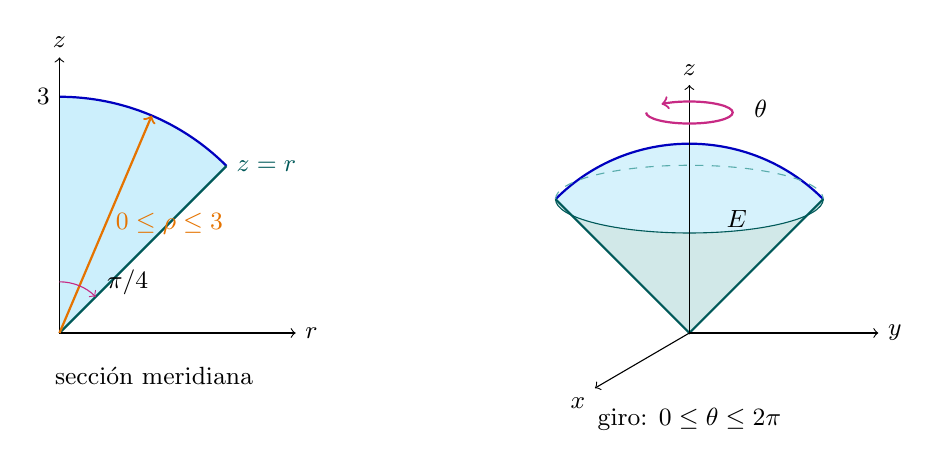
\begin{tikzpicture}[every node/.style={font=\small}]
    \begin{scope}
        \fill[cyan!20] (0,0) -- (0,3) arc[start angle=90,end angle=45,radius=3] -- cycle;
        \draw[blue!75!black,thick] (0,3) arc[start angle=90,end angle=45,radius=3];
        \draw[teal!70!black,thick] (0,0) -- (2.12,2.12) node[right] {$z=r$};
        \draw[->] (0,0) -- (3,0) node[right] {$r$};
        \draw[->] (0,0) -- (0,3.5) node[above] {$z$};
        \draw[->,orange!90!black,thick] (0,0) -- ({3*sin(23)},{3*cos(23)})
            node[midway,right] {$0\leq\rho\leq3$};
        \draw[->,magenta!80!black] (0,.65) arc[start angle=90,end angle=45,radius=.65];
        \node[right] at (.48,.65) {$\pi/4$};
        \node[left] at (0,3) {$3$};
        \node at (1.2,-.55) {sección meridiana};
    \end{scope}
    \begin{scope}[xshift=8cm]
        \fill[cyan!16] (0,0) -- (-1.7,1.7) arc[start angle=135,end angle=45,radius=2.404] -- cycle;
        \fill[teal!18] (0,0) -- (-1.7,1.7)
            arc[start angle=180,end angle=360,x radius=1.7,y radius=.43] -- cycle;
        \draw[blue!75!black,thick] (-1.7,1.7) arc[start angle=135,end angle=45,radius=2.404];
        \draw[teal!70!black,thick] (-1.7,1.7) -- (0,0) -- (1.7,1.7);
        \draw[dashed,teal!65] (-1.7,1.7) arc[start angle=180,end angle=0,x radius=1.7,y radius=.43];
        \draw[teal!70!black] (-1.7,1.7) arc[start angle=180,end angle=360,x radius=1.7,y radius=.43];
        \draw[->] (0,0) -- (2.4,0) node[right] {$y$};
        \draw[->] (0,0) -- (-1.2,-.7) node[below left] {$x$};
        \draw[->] (0,0) -- (0,3.15) node[above] {$z$};
        \draw[->,magenta!80!black,thick] (-.55,2.8)
            arc[start angle=180,end angle=490,x radius=.55,y radius=.14];
        \node[right] at (.7,2.85) {$\theta$};
        \node at (.6,1.45) {$E$};
        \node at (0,-1.1) {giro: $0\leq\theta\leq2\pi$};
    \end{scope}
\end{tikzpicture}
\end{center}
\endgroup

Por tanto,
\begin{align*}
V&=\int_0^{2\pi}\int_0^{\pi/4}\int_0^3
\rho^2\sin\varphi\,d\rho\,d\varphi\,d\theta\\
&=\int_0^{2\pi}\int_0^{\pi/4}9\sin\varphi\,d\varphi\,d\theta
=18\pi\left(1-\frac{\sqrt2}{2}\right).
\end{align*}

\paragraph{Ejemplo 2. Masa de una esfera con densidad radial}

Una esfera maciza de radio $R>0$, centrada en el origen, tiene densidad
\[
\rho_m(x,y,z)=\rho_0\left(1+\frac{x^2+y^2+z^2}{R^2}\right),
\qquad \rho_0>0.
\]
La densidad es constante sobre cada esfera concéntrica y aumenta desde $\rho_0$ en el centro hasta $2\rho_0$ en la superficie. En coordenadas esféricas se expresa como $\rho_m=\rho_0(1+\rho^2/R^2)$.

\begingroup
\shorthandoff{>}
\begin{center}
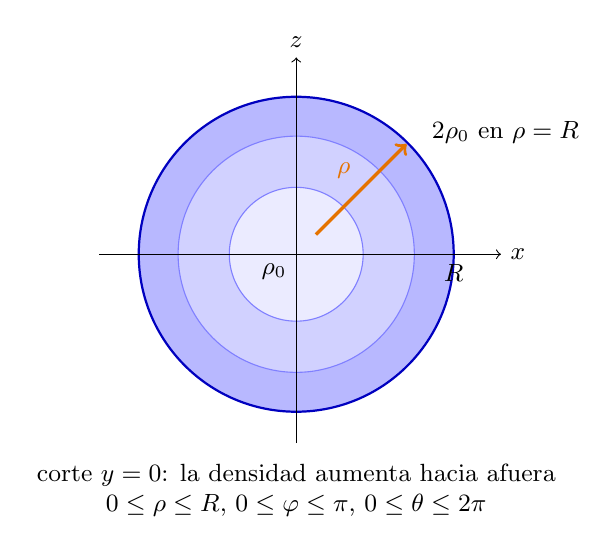
\begin{tikzpicture}[every node/.style={font=\small}]
    \fill[blue!28] (0,0) circle (2);
    \fill[blue!18] (0,0) circle (1.5);
    \fill[blue!8] (0,0) circle (.85);
    \draw[blue!75!black,thick] (0,0) circle (2);
    \foreach \rr in {.85,1.5} {\draw[blue!50] (0,0) circle (\rr);}
    \draw[->] (-2.5,0) -- (2.6,0) node[right] {$x$};
    \draw[->] (0,-2.4) -- (0,2.5) node[above] {$z$};
    \draw[->,orange!90!black,very thick] (.25,.25) -- (1.4,1.4)
        node[midway,above left] {$\rho$};
    \node[below left] at (0,0) {$\rho_0$};
    \node[right] at (1.6,1.55) {$2\rho_0$ en $\rho=R$};
    \node[below] at (2,0) {$R$};
    \node[align=center] at (0,-3) {corte $y=0$: la densidad aumenta hacia afuera\\$0\leq\rho\leq R$, $0\leq\varphi\leq\pi$, $0\leq\theta\leq2\pi$};
\end{tikzpicture}
\end{center}
\endgroup

La masa total es
\begin{align*}
m&=\rho_0\int_0^{2\pi}\int_0^\pi\int_0^R
\left(1+\frac{\rho^2}{R^2}\right)\rho^2\sin\varphi
\,d\rho\,d\varphi\,d\theta\\
&=\rho_0(2\pi)(2)
\left[\frac{\rho^3}{3}+\frac{\rho^5}{5R^2}\right]_0^R
=\frac{32\pi\rho_0R^3}{15}.
\end{align*}
Como $V=4\pi R^3/3$, la densidad media es $m/V=8\rho_0/5$, que se encuentra entre los valores mínimo y máximo de la densidad.

\paragraph{Ejemplo 3. Centro de masa de una semiesfera homogénea}

Se considera la semiesfera maciza superior
\[
E=\{(x,y,z):x^2+y^2+z^2\leq R^2,\ z\geq0\},
\qquad R>0,
\]
con densidad constante $\rho_m=\rho_0>0$. Sus cotas son
\[
0\leq\rho\leq R,\qquad 0\leq\varphi\leq\pi/2,
\qquad 0\leq\theta\leq2\pi.
\]

\begingroup
\shorthandoff{>}
\begin{center}
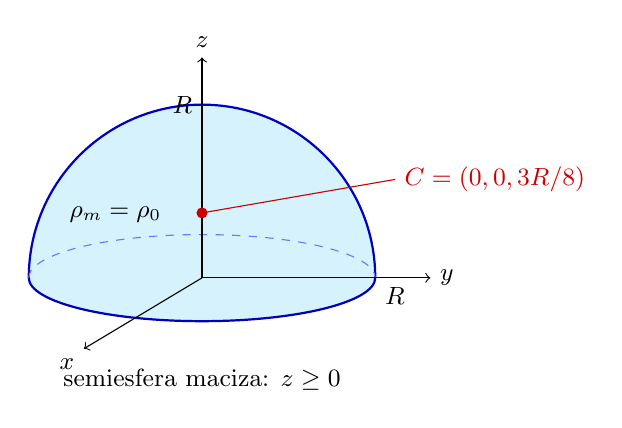
\begin{tikzpicture}[every node/.style={font=\small}]
    \fill[cyan!16] (-2.2,0) arc[start angle=180,end angle=0,radius=2.2]
        arc[start angle=0,end angle=-180,x radius=2.2,y radius=.55] -- cycle;
    \draw[blue!75!black,thick] (-2.2,0) arc[start angle=180,end angle=0,radius=2.2];
    \draw[dashed,blue!55] (-2.2,0) arc[start angle=180,end angle=0,x radius=2.2,y radius=.55];
    \draw[blue!75!black,thick] (-2.2,0) arc[start angle=180,end angle=360,x radius=2.2,y radius=.55];
    \draw[->] (0,0) -- (2.9,0) node[right] {$y$};
    \draw[->] (0,0) -- (-1.5,-.9) node[below left] {$x$};
    \draw[->] (0,0) -- (0,2.8) node[above] {$z$};
    \node[left] at (0,2.2) {$R$};
    \fill[red!80!black] (0,.825) circle (2pt);
    \draw[red!80!black] (0,.825) -- (2.45,1.25)
        node[right] {$C=(0,0,3R/8)$};
    \node at (-1.1,.8) {$\rho_m=\rho_0$};
    \node[below right] at (2.2,0) {$R$};
    \node at (0,-1.3) {semiesfera maciza: $z\geq0$};
\end{tikzpicture}
\end{center}
\endgroup

Las reflexiones $x\mapsto-x$ e $y\mapsto-y$ conservan el sólido y su densidad. Por tanto, los primeros momentos $M_{yz}$ y $M_{xz}$ se anulan y $\bar x=\bar y=0$. Para la coordenada restante se calculan la masa y el momento respecto de $xy$:
\begin{align*}
m&=\rho_0\int_0^{2\pi}\int_0^{\pi/2}\int_0^R
\rho^2\sin\varphi\,d\rho\,d\varphi\,d\theta
=\frac{2\pi\rho_0R^3}{3},\\
M_{xy}&=\iiint_E z\rho_0\,dV\\
&=\rho_0\int_0^{2\pi}\int_0^{\pi/2}\int_0^R
\rho^3\cos\varphi\sin\varphi\,d\rho\,d\varphi\,d\theta\\
&=\rho_0(2\pi)\frac{R^4}{4}
\left[\frac{\sin^2\varphi}{2}\right]_0^{\pi/2}
=\frac{\pi\rho_0R^4}{4}.
\end{align*}
En consecuencia,
\[
\bar z=\frac{M_{xy}}m=\frac{3R}{8},\qquad
(\bar x,\bar y,\bar z)=\left(0,0,\frac{3R}{8}\right).
\]

\subsection{Ejercicios}
\begin{enumerate}
    \item Evalúa
\[
\int_0^{2\pi}\int_0^2\int_0^3 (r^2+z)r\,dz\,dr\,d\theta.
\]

    \item Evalúa
\[
\int_0^{\pi/2}\int_0^\pi\int_1^2
\rho^4\sin\varphi\,d\rho\,d\varphi\,d\theta.
\]

    \item Evalúa
\[
\int_0^\pi\int_0^1\int_{r^2}^{2-r^2}
zr\,dz\,dr\,d\theta.
\]

    \item Evalúa
\[
\int_0^{2\pi}\int_0^{\pi/3}\int_0^2
\rho^3\cos\varphi\sin\varphi\,d\rho\,d\varphi\,d\theta.
\]

    \item Grafica la región de integración de
\[
\int_0^{\pi/2}\int_1^2\int_0^3 r\,dz\,dr\,d\theta.
\]

    \item Grafica la región de integración de
\[
\int_0^{2\pi}\int_{\pi/4}^{\pi/2}\int_1^3
\rho^2\sin\varphi\,d\rho\,d\varphi\,d\theta.
\]

    \item Grafica la región de integración de
\[
\int_{-\pi/2}^{\pi/2}\int_0^{2\cos\theta}\int_0^{r^2}
r\,dz\,dr\,d\theta.
\]

    \item Grafica la región de integración de
\[
\int_0^{2\pi}\int_0^{\pi/2}\int_0^{4\cos\varphi}
\rho^2\sin\varphi\,d\rho\,d\varphi\,d\theta.
\]

    \item Convierte a coordenadas cilíndricas y evalúa
\[
\int_{-2}^2\int_{-\sqrt{4-x^2}}^{\sqrt{4-x^2}}
\int_0^{4-x^2-y^2}(x^2+y^2)\,dz\,dy\,dx.
\]

    \item Convierte a coordenadas esféricas y evalúa
\[
\int_{-2}^2\int_{-\sqrt{4-x^2}}^{\sqrt{4-x^2}}
\int_0^{\sqrt{4-x^2-y^2}}
(x^2+y^2+z^2)\,dz\,dy\,dx.
\]
    
    \item Convierte a coordenadas cilíndricas y evalúa
\[
\int_0^2\int_{-\sqrt{2x-x^2}}^{\sqrt{2x-x^2}}
\int_0^{\sqrt{x^2+y^2}}1\,dz\,dy\,dx.
\]

    \item Convierte a coordenadas esféricas y evalúa
\[
\int_0^{2\pi}\int_0^{\sqrt2}\int_r^{\sqrt{4-r^2}}
z\sqrt{r^2+z^2}\,r\,dz\,dr\,d\theta.
\]

    \item Formula y evalúa la integral triple para el volumen del sólido $E$ representado en la figura.

\begingroup
\shorthandoff{>}
\begin{center}
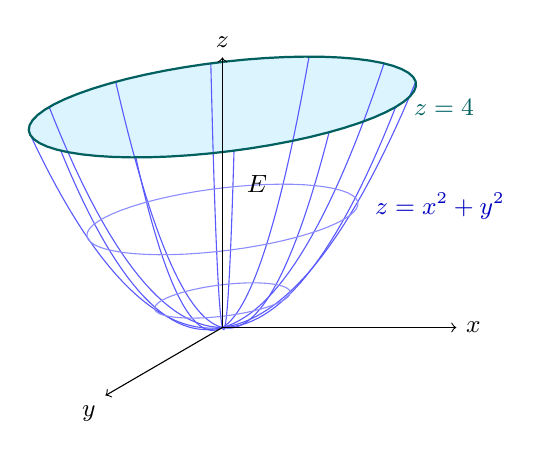
\begin{tikzpicture}[x={(1.1cm,0cm)},y={(-.55cm,-.32cm)},z={(0cm,.7cm)},every node/.style={font=\small}]
    \fill[cyan!14] plot[domain=0:360,samples=60] ({2*cos(\x)},{2*sin(\x)},4) -- cycle;
    \foreach \tt in {0,30,...,330} {
        \draw[blue!65] plot[domain=0:2,samples=30] ({\x*cos(\tt)},{\x*sin(\tt)},{\x*\x});
    }
    \foreach \rr in {.7,1.4} {
        \draw[blue!45] plot[domain=0:360,samples=60] ({\rr*cos(\x)},{\rr*sin(\x)},{\rr*\rr});
    }
    \draw[teal!75!black,thick] plot[domain=0:360,samples=60] ({2*cos(\x)},{2*sin(\x)},4);
    \draw[->] (0,0,0) -- (2.7,0,0) node[right] {$x$};
    \draw[->] (0,0,0) -- (0,2.7,0) node[below left] {$y$};
    \draw[->] (0,0,0) -- (0,0,4.9) node[above] {$z$};
    \node[right,teal!75!black] at (2.1,0,4) {$z=4$};
    \node[right,blue!75!black] at (1.65,0,2.2) {$z=x^2+y^2$};
    \node at (.4,0,2.6) {$E$};
\end{tikzpicture}
\end{center}
\endgroup

    \item Formula y evalúa $\iiint_E z\,dV$ para el sólido representado en la figura.

\begingroup
\shorthandoff{>}
\begin{center}
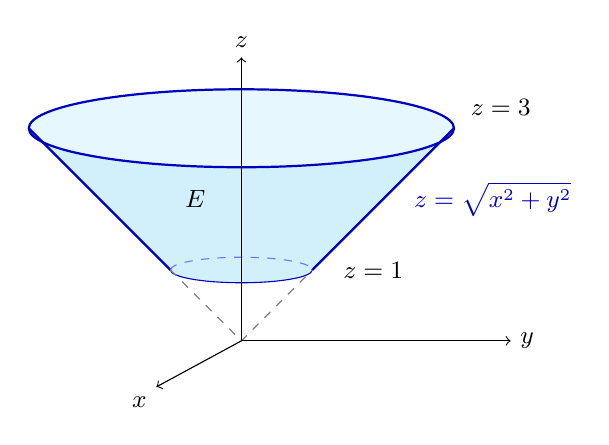
\begin{tikzpicture}[every node/.style={font=\small},scale=.9]
    \fill[cyan!18] (-1,1) -- (-3,3)
        arc[start angle=180,end angle=360,x radius=3,y radius=.55]
        -- (1,1) arc[start angle=0,end angle=-180,x radius=1,y radius=.18] -- cycle;
    \fill[cyan!10] (0,3) ellipse (3 and .55);
    \draw[blue!75!black,thick] (-1,1) -- (-3,3) (1,1) -- (3,3);
    \draw[blue!75!black,thick] (0,3) ellipse (3 and .55);
    \draw[dashed,blue!55] (-1,1) arc[start angle=180,end angle=0,x radius=1,y radius=.18];
    \draw[blue!75!black] (-1,1) arc[start angle=180,end angle=360,x radius=1,y radius=.18];
    \draw[dashed,gray] (-1,1) -- (0,0) -- (1,1);
    \draw[->] (0,0) -- (3.8,0) node[right] {$y$};
    \draw[->] (0,0) -- (-1.2,-.65) node[below left] {$x$};
    \draw[->] (0,0) -- (0,4) node[above] {$z$};
    \node[right] at (3.1,3.3) {$z=3$};
    \node[right] at (1.3,1) {$z=1$};
    \node[right,blue!75!black] at (2.3,2) {$z=\sqrt{x^2+y^2}$};
    \node at (-.65,2) {$E$};
\end{tikzpicture}
\end{center}
\endgroup

    \item El sólido $E$ se obtiene al girar la región sombreada una vuelta completa alrededor del eje $z$. Evalúa
\[
\iiint_E (x^2+y^2+z^2)\,dV.
\]

\begingroup
\shorthandoff{>}
\begin{center}
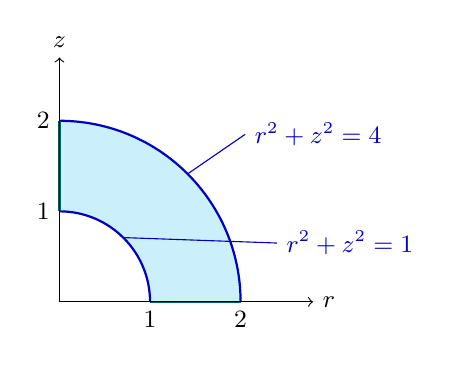
\begin{tikzpicture}[every node/.style={font=\small},scale=1.15]
    \fill[cyan!20] (0,2) arc[start angle=90,end angle=0,radius=2]
        -- (1,0) arc[start angle=0,end angle=90,radius=1] -- cycle;
    \draw[blue!75!black,thick] (0,2) arc[start angle=90,end angle=0,radius=2];
    \draw[blue!75!black,thick] (1,0) arc[start angle=0,end angle=90,radius=1];
    \draw[teal!75!black,thick] (0,1) -- (0,2) (1,0) -- (2,0);
    \draw[->] (0,0) -- (2.8,0) node[right] {$r$};
    \draw[->] (0,0) -- (0,2.7) node[above] {$z$};
    \node[left] at (0,1) {$1$};
    \node[left] at (0,2) {$2$};
    \node[below] at (1,0) {$1$};
    \node[below] at (2,0) {$2$};
    \draw[blue!75!black] (1.41,1.41) -- (2.05,1.85) node[right] {$r^2+z^2=4$};
    \draw[blue!75!black] (.71,.71) -- (2.4,.65) node[right] {$r^2+z^2=1$};
\end{tikzpicture}
\end{center}
\endgroup

    \item El sólido $E$ se obtiene al girar la región sombreada una vuelta completa alrededor del eje $z$.
\begin{itemize}
    \item Evalúa la triple integral utilizando coordenadas cilíndricas.
    \item Evalúa la triple integral utilizando coordenadas esféricas.
\end{itemize}
Compara los resultados obtenidos con ambos sistemas de coordenadas.

\begingroup
\shorthandoff{>}
\begin{center}
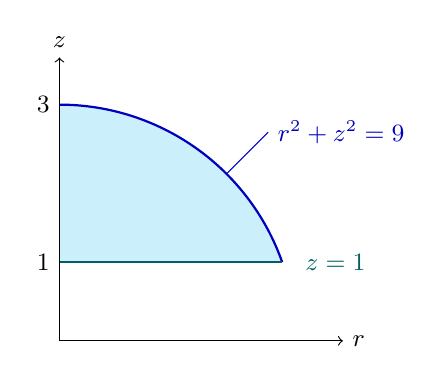
\begin{tikzpicture}[every node/.style={font=\small}]
    \fill[cyan!20] (0,1) -- (0,3)
        arc[start angle=90,end angle=19.47122,radius=3] -- cycle;
    \draw[blue!75!black,thick] (0,3)
        arc[start angle=90,end angle=19.47122,radius=3];
    \draw[teal!75!black,thick] (0,1) -- ({sqrt(8)},1);
    \draw[->] (0,0) -- (3.6,0) node[right] {$r$};
    \draw[->] (0,0) -- (0,3.6) node[above] {$z$};
    \node[left] at (0,1) {$1$};
    \node[left] at (0,3) {$3$};
    \node[right,teal!75!black] at (3,1) {$z=1$};
    \draw[blue!75!black] (2.12,2.12) -- (2.65,2.65)
        node[right] {$r^2+z^2=9$};
\end{tikzpicture}
\end{center}
\endgroup

\end{enumerate}
